%%%%%%%% ICML 2026 SUBMISSION (anonymized) %%%%%%%%%%%%%%%%%
%% gDTR: Layer-wise Settling Depth as an Interpretability Axis
%% for Genomic Causal Foundation Models
%% Submission to the ICML 2026 Workshop on Interpretable Machine
%% Learning in the Sciences (short paper: 4 pages + appendix)

\documentclass{article}

% Recommended, but optional, packages for figures and better typesetting:
\usepackage{microtype}
\usepackage{graphicx}
\usepackage{subcaption}
\usepackage{booktabs}      % professional tables
\usepackage{multirow}
\usepackage{array}
\usepackage{siunitx}       % aligned numerics in tables
\usepackage{xcolor}

\usepackage{hyperref}
\newcommand{\theHalgorithm}{\arabic{algorithm}}

% Use the following line for the initial blind version submitted for review:
\usepackage{icml2026}

% For preprint, use
% \usepackage[preprint]{icml2026}

% If accepted, instead use the following line for the camera-ready submission:
% \usepackage[accepted]{icml2026}

\usepackage{amsmath}
\usepackage{amssymb}
\usepackage{mathtools}
\usepackage{amsthm}

% if you use cleveref..
\usepackage[capitalize,noabbrev]{cleveref}

%%%%%%%%%%%%%%%%%%%%%%%%%%%%%%%%
% THEOREMS / DEFINITIONS
%%%%%%%%%%%%%%%%%%%%%%%%%%%%%%%%
\theoremstyle{plain}
\newtheorem{theorem}{Theorem}[section]
\newtheorem{proposition}[theorem]{Proposition}
\newtheorem{lemma}[theorem]{Lemma}
\newtheorem{corollary}[theorem]{Corollary}
\theoremstyle{definition}
\newtheorem{definition}[theorem]{Definition}
\newtheorem{assumption}[theorem]{Assumption}
\theoremstyle{remark}
\newtheorem{remark}[theorem]{Remark}

%%%%%%%%%%%%%%%%%%%%%%%%%%%%%%%%
% MACROS
%%%%%%%%%%%%%%%%%%%%%%%%%%%%%%%%
\newcommand{\gDTR}{\textsc{gDTR}}
\newcommand{\DTR}{\textsc{DTR}}
\newcommand{\hl}{h_{\ell}}
\newcommand{\hnorm}{h_{\mathrm{norm}}}
\newcommand{\Dcos}{D_{\cos}}
\newcommand{\Djsd}{D_{\mathrm{jsd}}}
\newcommand{\DDcos}{\Delta D_{\cos}}
\newcommand{\DDjsd}{\Delta D_{\mathrm{jsd}}}
\newcommand{\runmin}{\operatorname{run\text{-}min}}

% Running title (kept short for the page header)
\icmltitlerunning{gDTR: Layer-wise Settling Depth for Genomic Causal Foundation Models}

\begin{document}

\twocolumn[
  \icmltitle{\gDTR{}: Layer-wise Settling Depth as an Interpretability Axis\\
             for Genomic Causal Foundation Models}

  % Anonymous submission (the [accepted] option is OFF, so the style file
  % will hide author info automatically). We still list dummy authors so the
  % author block does not collapse into the abstract.
  \icmlsetsymbol{equal}{*}

  \begin{icmlauthorlist}
    \icmlauthor{Anonymous Authors}{anon}
  \end{icmlauthorlist}

  \icmlaffiliation{anon}{Anonymous Institution}
  \icmlcorrespondingauthor{Anonymous Authors}{anonymous@example.org}

  \icmlkeywords{Interpretability, Genomic Foundation Models,
                Logit Lens, Tuned Lens, Mutational Signatures,
                Variant Effect Prediction, Mechanistic Interpretability}

  \vskip 0.3in
]

% No special notice (required even if empty).
\printAffiliationsAndNotice{}

%%%%%%%%%%%%%%%%%%%%%%%%%%%%%%%%
% ABSTRACT
%%%%%%%%%%%%%%%%%%%%%%%%%%%%%%%%
\begin{abstract}
We introduce \gDTR{} (\emph{Genomic Deep-Thinking Ratio}), a training-free, layer-resolved interpretability framework for genomic causal foundation models. \gDTR{} measures, for every nucleotide token, the \emph{settling depth} $c(t)$ -- the layer at which intermediate predictions stabilise on the final-layer distribution -- through a cosine unembed-residual lens with running-minimum convergence. On Evo~2~7B, $c(t)$ exposes a chr22-calibrated / chr17-validated splice-shallow universality, generalises to a shallowness signature at ENCODE cCRE-ELS regulatory elements, and yields class-stratified disruption layers across 4{,}023 ClinVar P/LP variants ($p=7\!\times\!10^{-10}$). \gDTR{} thus complements attention-based, dictionary-based, and output-side interpretability tools with a fourth, hierarchical axis: \emph{where, in the layer stack, biology is recognised}.
\end{abstract}

%%%%%%%%%%%%%%%%%%%%%%%%%%%%%%%%
% Fig 1 — schematic (top of paper)
%%%%%%%%%%%%%%%%%%%%%%%%%%%%%%%%
\begin{figure*}[!t]
\centering
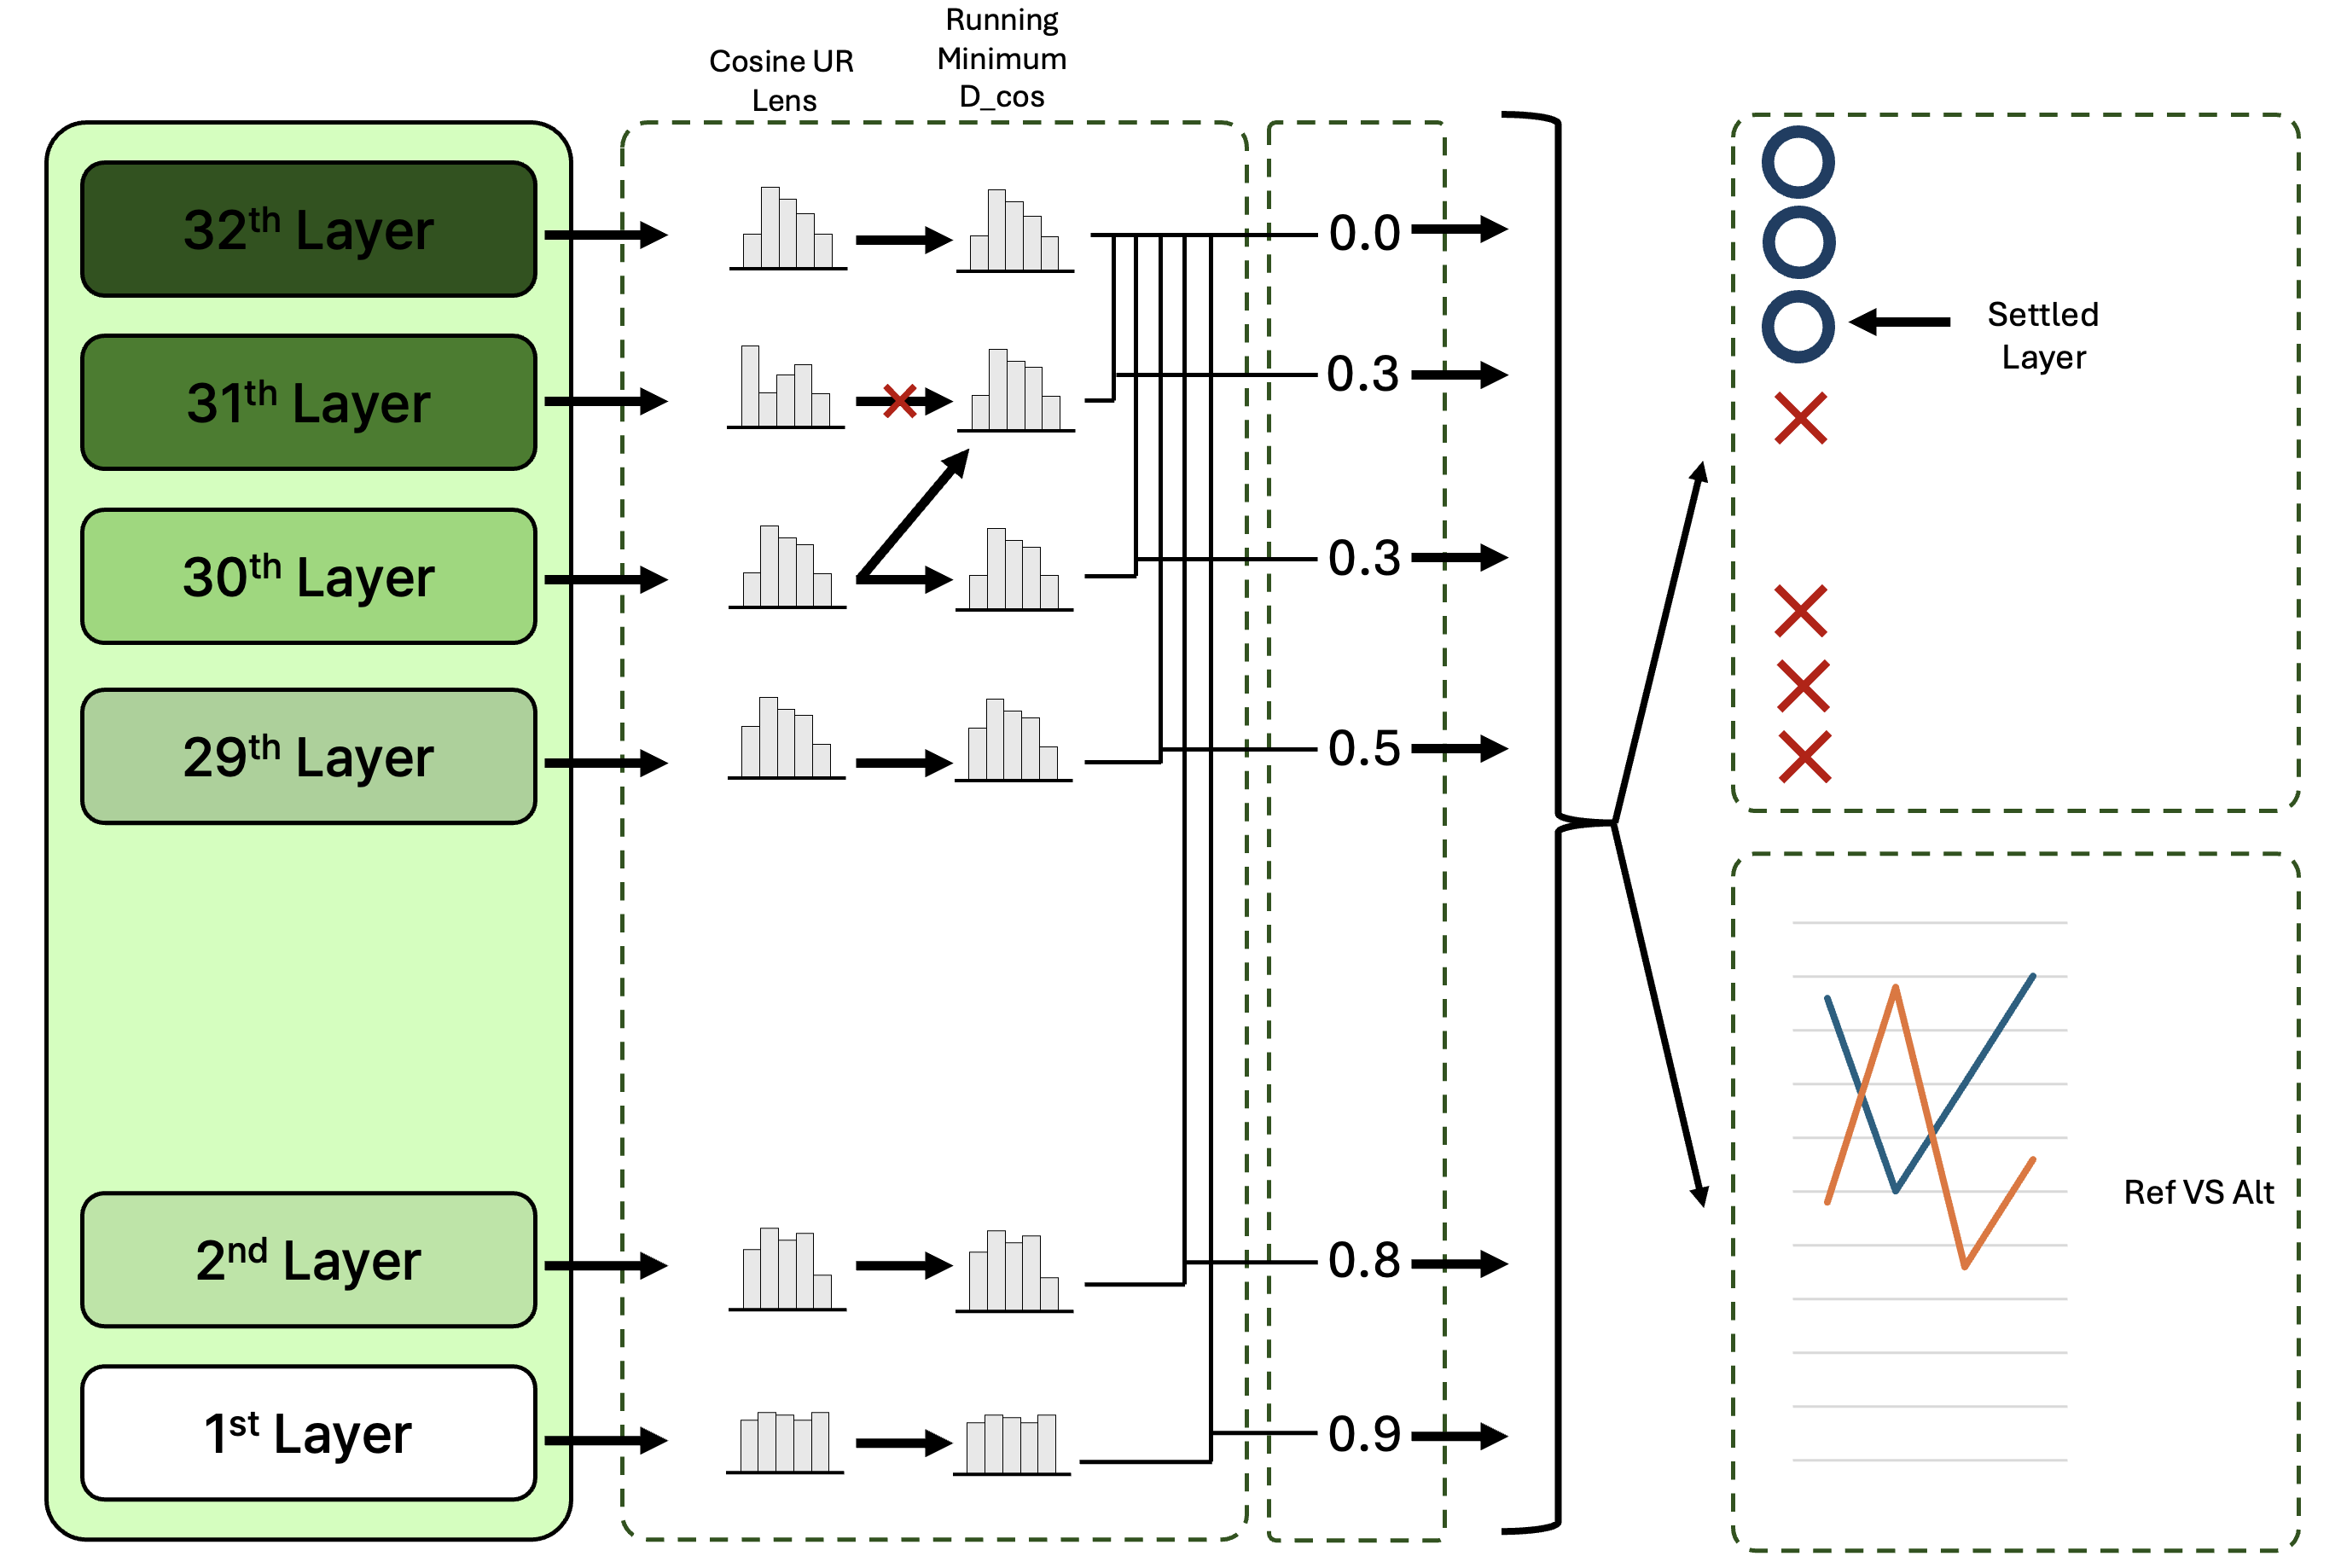
\includegraphics[width=0.78\textwidth]{figures/fig_schematic.png}
\caption{\gDTR{} pipeline. For each token, the cosine unembed-residual (UR) lens computes a per-layer distance $\Dcos(\ell,t) = 1-\cos(\hl(t),\hnorm(t))$ between the residual stream and the post-final-norm reference. A running minimum (envelope) collapses architecture-specific non-monotonicity, and the first $\ell$ at which the envelope crosses $\gamma_{\cos}$ (regional $q_{70}$ calibration) is the \emph{settling depth} $c(t)$ -- the ``settled layer''. On a variant we apply the same machinery to the reference and alternate sequences and read the per-layer $\DDcos$ trajectory to localise the maximum-disruption layer.}
\label{fig:schematic}
\end{figure*}

%%%%%%%%%%%%%%%%%%%%%%%%%%%%%%%%
% 1. INTRODUCTION
%%%%%%%%%%%%%%%%%%%%%%%%%%%%%%%%
\section{Introduction}
\label{sec:intro}

Genomic causal foundation models such as Evo~2 \cite{nguyen2026evo2}, HyenaDNA~\cite{nguyen2023hyenadna}, the Nucleotide Transformer~\cite{dallatorre2024nt}, DNABERT-2~\cite{zhou2024dnabert2}, and Caduceus~\cite{schiff2024caduceus} have catalysed a paradigm shift in functional genomics. Yet research into their internal mechanisms still lags: the layer-wise computational dynamics of these models remain largely opaque, leaving open the question of whether their outputs are grounded in biology that a human geneticist would recognise. Existing tools probe \emph{where} models attend (attention rollout~\cite{abnar2020rollout}, Enformer-style attribution~\cite{avsec2021enformer}), \emph{what} they encode (sparse dictionaries~\cite{bricken2023monosemanticity,cunningham2023sparse}), or \emph{how} variants shift representations (output-side $\Delta\textrm{LL}$, AlphaMissense~\cite{cheng2023alphamissense}, SpliceAI~\cite{jaganathan2019spliceai}). None addresses \emph{where in the layer hierarchy} a biological element is recognised.

We introduce a fourth, hierarchical axis. The Deep-Thinking Ratio of~\citet{chen2026deepthinking} measures, in NLP transformers, the layer index at which intermediate logit-lens distributions~\cite{nostalgebraist2020logitlens,belrose2023tunedlens,pal2023futurelens} converge within $\varepsilon$ of the final layer; the construct echoes the broader observation that mid-stack layers carry interpretable factual content~\cite{geva2022ffn,meng2022rome}. Genomic CLMs, however, demand three non-trivial adaptations:
\begin{itemize}
  \item \textbf{Small vocabulary.} With $|V|\!\le\!512$ (often 12), Jensen--Shannon divergence saturates and loses dynamic range; we replace it with a cosine unembed-residual lens.
  \item \textbf{Architecture diversity.} StripedHyena~\cite{poli2023striped}, pure Hyena~\cite{poli2023hyena}, and Transformer-MLM~\cite{vaswani2017attention} backbones each induce non-monotonic per-layer convergence, which we tame with a running-minimum envelope.
  \item \textbf{Final-block idleness.} In Evo~2 the last attention block is a residual passthrough (App.~\ref{app:architectural-quirk}); the canonical ``tap the last block'' convention breaks, so we calibrate against the post-final-norm reference and lock the canonical tap at $L^\star\!=\!29$.
\end{itemize}
The full pipeline is summarised in Fig.~\ref{fig:schematic}.


%%%%%%%%%%%%%%%%%%%%%%%%%%%%%%%%
% 2. FRAMEWORK

%%%%%%%%%%%%%%%%%%%%%%%%%%%%%%%%
% 2. FRAMEWORK
%%%%%%%%%%%%%%%%%%%%%%%%%%%%%%%%
\section{The \gDTR{} Framework}
\label{sec:framework}

For a nucleotide sequence of length $T$ processed by a causal language model with $L$ layers, we extract the residual-stream activation $\hl(t)$ at every layer $\ell\!\in\!\{1,\ldots,L\}$ and token position $t$. We replace the JSD lens of the parent DTR~\cite{chen2026deepthinking} with a cosine unembed-residual lens that operates directly in hidden-state geometry,
\begin{equation}
  \Dcos(\ell, t) \;=\; 1 - \cos\!\bigl(\hl(t),\, \hnorm(t)\bigr),
  \label{eq:cos-lens}
\end{equation}
where $\hnorm(t)$ is the post-final-norm reference. Whereas NLP transformers exhibit near-monotonic logit-lens convergence~\cite{nostalgebraist2020logitlens,belrose2023tunedlens}, genomic CLMs do not (Hyena alignment rotations, Evo~2 idle final block). We therefore define the \emph{settling depth} via a running-minimum envelope,
\begin{equation}
  c(t) \;=\; \min\bigl\{\, \ell \;:\; \runmin\,\Dcos(\ell, t) \le \gamma_{\cos}\bigr\},
  \label{eq:settling}
\end{equation}
with $\runmin\,\Dcos(\ell,t) = \min_{k\le\ell}\Dcos(k,t)$. The threshold $\gamma_{\cos}$ is set by \emph{regional $q_{70}$ calibration}: the 70th percentile of the running-min cosine-distance at the penultimate layer over the analysis region. The 70th percentile sits inside a flat plateau of a $5\!\times\!5$ grid sweep over $(\gamma_{\cos},\rho)$ (App.~\ref{app:gamma-sweep}; SD across 25 cells $<0.04$). The original deep-thinking ratio $\mathrm{DTR}(t)\!=\!\mathbf{1}\{c(t) \!>\! \rho L\}$ follows directly with $\rho\!=\!0.85$.

\paragraph{Tuned-lens recovery (training-free).} A per-layer affine fit~\cite{belrose2023tunedlens} reaches $\ge 98\%$ MSE recovery on $30/32$ Evo~2 layers (canonical $L^\star\!=\!29$: $0.9996$; App.~\ref{app:tuned-lens}), so no learned weights are required at inference and \gDTR{} remains training-free.


%%%%%%%%%%%%%%%%%%%%%%%%%%%%%%%%
% 3. BIOLOGICAL UTILITY
%%%%%%%%%%%%%%%%%%%%%%%%%%%%%%%%
\section{Biological Utility}
\label{sec:utility}

\subsection{Genome-wide shallowness signature}
\label{sec:shallowness}

We first ask whether $c(t)$ delivers a biologically meaningful, transferable readout at the genome scale. Chromosome~22 serves as the calibration set ($\gamma_{\cos}\!=\!0.397$ from $q_{70}$ at the penultimate layer); chromosome~17 is held out for validation with that $\gamma$ frozen. The chr17 $q_{70}$ recomputed independently equals $0.394$ ($|\Delta|\!=\!0.0023$): the calibration transfers without re-tuning, and chr17 reproduces the chr22 splice-donor effect (Cohen's $d\!=\!-0.349$ vs intron, $94.6\%$ of the chr22 magnitude $-0.369$).

\textbf{Splice universality.} On the seven canonical genomic contexts (Fig.~\ref{fig:shallowness}a), splice donor and acceptor sites converge $\sim 2$ layers earlier than the intronic baseline, while every non-splice context (3$'$ UTR, coding exon, intergenic, 5$'$ UTR) is at or above the baseline. The effect is monotone in donor/acceptor magnitude and statistically significant against intron at every context (Mann–Whitney $p\!<\!10^{-4}$ for all rows). A finer dissection by motif class (canonical GT-AG, canonical GC-AG, non-canonical) preserves the universality-vs-intron inequality but reverses the within-class ordering relative to the naive ``stronger motif $\Rightarrow$ shallower recognition'' prior~\cite{wang2008splicecode,yeo2004maxentscan,burge1998u12}, with non-canonical donors converging earliest and GC-AG canonical donors deepest (App.~\ref{app:splice-canonical}).

\textbf{Functional generalisation.} The same shallowness axis extends to known regulatory elements (Fig.~\ref{fig:shallowness}b). On chr22, ENCODE cCRE-ELS enhancer-like elements~\cite{moore2020encode} are shallower than a per-position background by Cohen's $d\!=\!-0.190$ ($p_{\textrm{Bonf}}\!<\!10^{-4}$), against the splice-donor reference of $d\!=\!-0.433$. GTEx eQTLs~\cite{gtex2020} ($d\!=\!-0.022$) and GWAS Catalog SNPs~\cite{sollis2023gwas} ($d\!=\!-0.040$) sit on the same axis at biologically marginal magnitudes; their formal significance, when it appears, follows from the very large $n$. The unifying signal is that the model recognises well-characterised cis-elements in the first few layers, generalising the splice-shallow finding to the broader regulatory landscape.

\begin{figure*}[!t]
\centering
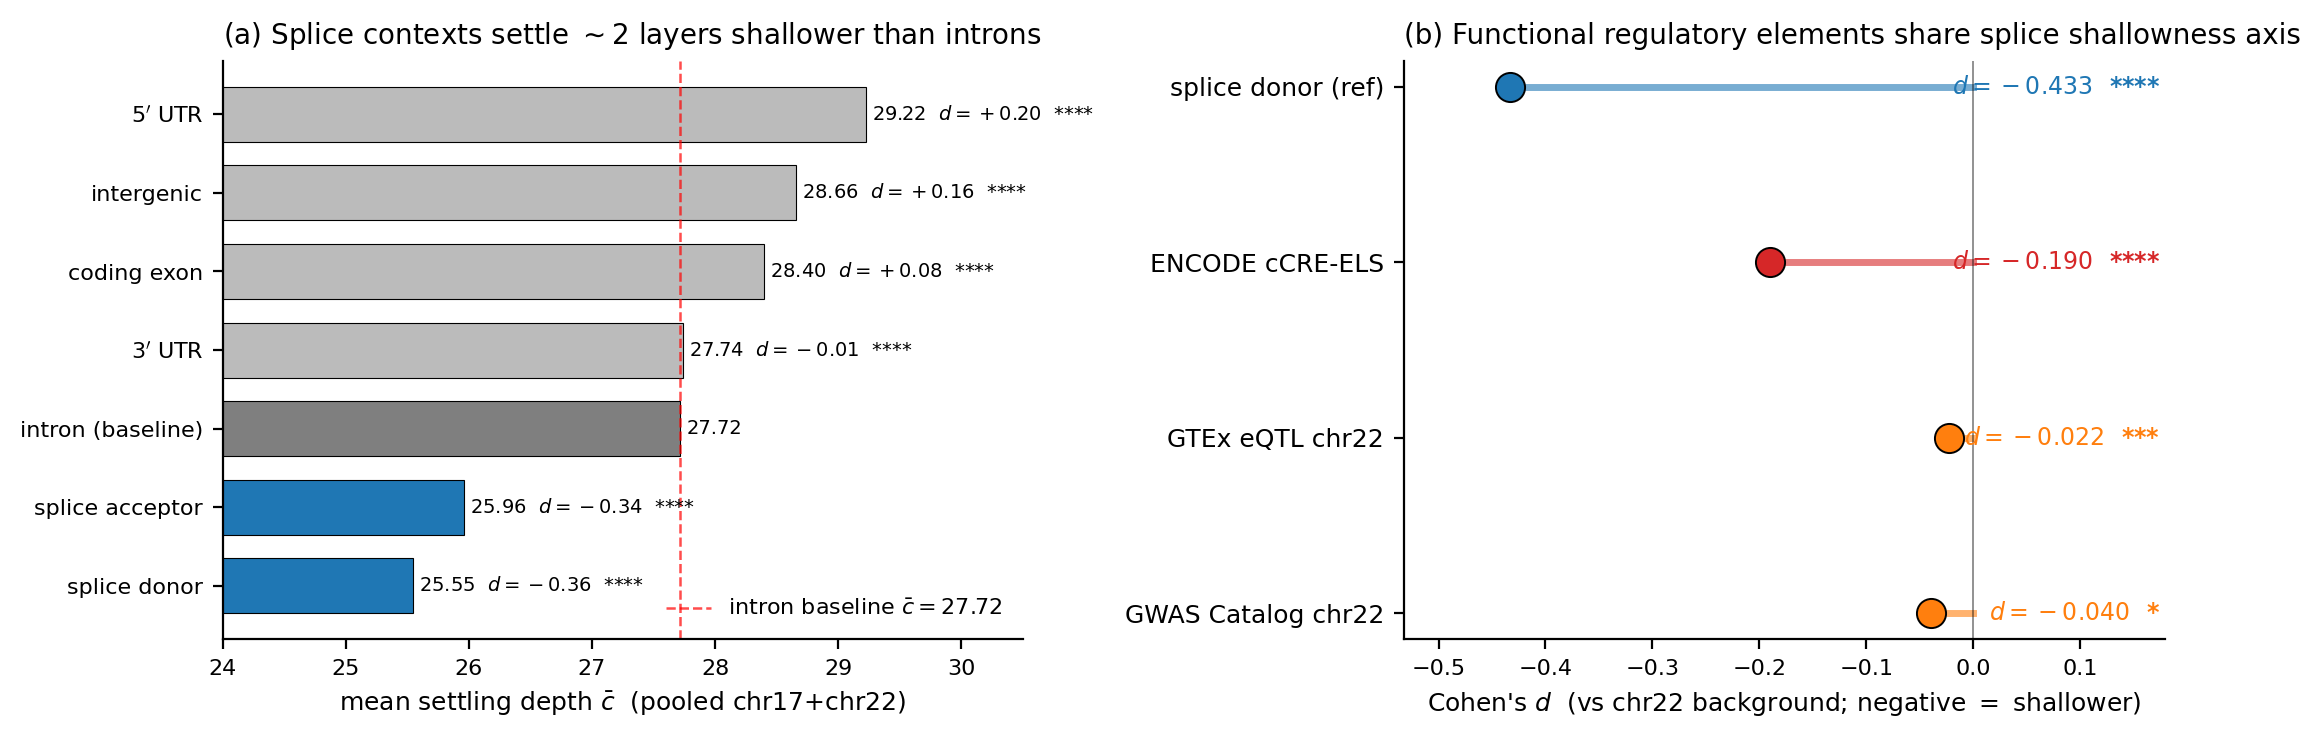
\includegraphics[width=0.95\textwidth]{figures/fig_shallowness.png}
\caption{Genome-wide shallowness signature. \textbf{(a)} Per-context mean settling depth $\bar c$ pooled over chr17 (validation, frozen $\gamma_{\cos}\!=\!0.397$) and chr22 (calibration). Splice donor and acceptor (blue) sit $\sim 2$ layers below the intron baseline (red dashed); all other contexts cluster at or above the baseline. Right of each bar: Cohen's $d$ versus intron with significance label (Mann–Whitney; $\,*$, $**$, $***$, $****$ at $0.05$, $0.01$, $10^{-3}$, $10^{-4}$). \textbf{(b)} Cohen's $d$ versus a chr22 per-position background for splice donor (reference; $-0.433$), ENCODE cCRE-ELS ($-0.190$), GTEx eQTL ($-0.022$) and GWAS Catalog ($-0.040$). $p$-values are Bonferroni-corrected over the four tests. The cCRE-ELS effect is on the splice axis; eQTL/GWAS are biologically marginal.}
\label{fig:shallowness}
\end{figure*}


\subsection{Layer-wise mechanistic analysis of variant disruption}
\label{sec:variant-disruption}

While $c(t)$ summarises shallowness at the genome scale, the per-variant argmax-layer of $|\DDcos|$ asks at what depth a single substitution maximally perturbs the residual stream. We test this on the full ClinVar~\cite{landrum2020clinvar} 15-cancer-gene cohort: $10{,}910$ SNVs (cached features) augmented by $1{,}064$ indels forwarded with the same Evo~2~7B pipeline (the SNV cache had silently filtered indels in the original Phase~3 run). Variants are class-stratified using ClinVar \texttt{MC} priorities (canonical-splice $\succ$ nonsense $\succ$ frameshift $\succ$ missense $\succ$ synonymous $\succ$ intron).

The argmax-layer medians order \emph{intron $<$ frameshift $<$ nonsense $<$ missense $\approx$ canonical splice $<$ synonymous} (Fig.~\ref{fig:variants}, top), differing across the six classes at Kruskal--Wallis $p\!=\!3.0\!\times\!10^{-10}$~\cite{kruskal1952wallis}. Adjacent-pair Dunn--Bonferroni tests~\cite{mann1947whitney,benjamini1995fdr} highlight the single largest jump as nonsense $\to$ missense ($p_{\textrm{adj}}\!<\!10^{-3}$); the remaining adjacent gaps are within noise on these per-class sample sizes ($n\!=\!32$--$1740$). Mechanistically, early-truncation events (frameshift, nonsense) disrupt the residual stream shallowly, whereas perturbations of already-established protein-level features (missense, splice motif) peak deeper. Five representative $\DDcos$ traces, one per non-intron class at the per-class median argmax-layer, are shown in Fig.~\ref{fig:variants}, bottom; the variant labelled ``frameshift locus'' in earlier drafts (\emph{BRCA1} 17:43{,}057{,}063 G$\to$A) is in fact a nonsense SNV (BRCA1 W1837X) and is now correctly classed.

\begin{figure*}[!t]
\centering
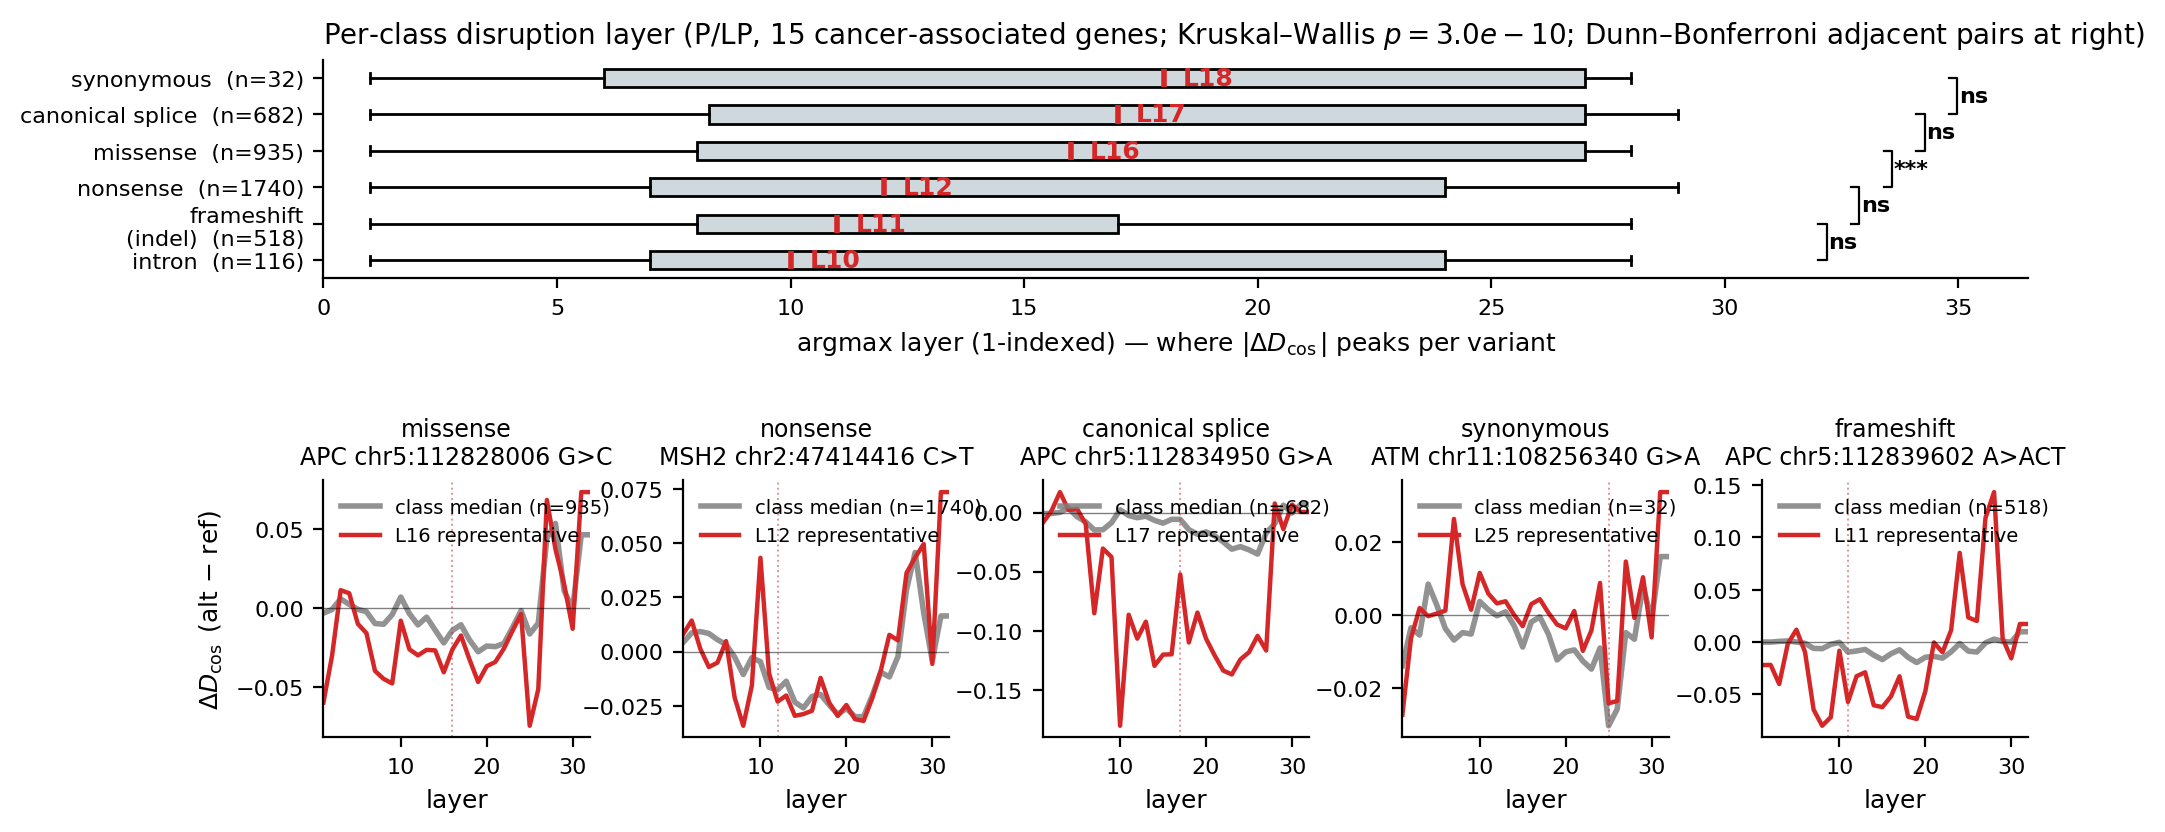
\includegraphics[width=0.98\textwidth]{figures/fig_variants.png}
\caption{Per-class disruption layer across $4{,}023$ ClinVar P/LP variants in 15 cancer-associated genes. \textbf{Top:} horizontal box plot of argmax layer of $|\DDcos|$ per molecular consequence class (intron / frameshift / nonsense / missense / canonical splice / synonymous). The class-median layer is annotated above each box. Kruskal--Wallis 6-way $p\!=\!3.0\!\times\!10^{-10}$; adjacent-pair Dunn--Bonferroni significance brackets at the right margin. \textbf{Bottom:} five representative $\DDcos$ traces, one per non-intron class, picked at the per-class median argmax layer (grey: per-class median trace; red: representative variant; dotted vertical: representative argmax). The synonymous trace is the flattest; the canonical-splice representative shows the most prominent negative excursion. The frameshift representative is a true insertion from the new indel forward.}
\label{fig:variants}
\end{figure*}

A logistic regression on the full 32-dimensional $\DDcos$ trajectory reaches stratified 10-fold AUROC $0.844$ ($95\%$ CI $[0.831, 0.857]$) on $8{,}008$ ClinVar P/LP-vs-B/LB SNVs across the same 15 genes, dominating the best single-layer tap ($\ell\!=\!30$, AUROC $0.729$) and the Evo~2 output-side $\Delta\textrm{LL}$ ($0.751$); leave-one-gene-out AUROC stays at $0.843$, and ensembling with $\Delta\textrm{LL}$ yields $0.861$. Full per-feature numbers, ROC curves, DeLong~\cite{delong1988comparing} pairwise tests, and the per-layer ablation are deferred to App.~\ref{app:auroc-detail} and App.~\ref{app:per-layer}; the headline is that the trajectory carries information beyond any single layer or output-side scalar.


\subsection{Cross-architecture invariance is two-tier, not universal}
\label{sec:cross-arch}

Extending the same chr22 windows to four genomic foundation models with divergent backbones (Evo~2~7B, HyenaDNA-large, NT-v2~500M, DNABERT-2; details in App.~\ref{app:fm-specs}) reveals a two-tier invariance rather than a universal one (App.~\ref{app:cross-arch} \&~\ref{app:crossarch-fig}): within the per-position causal-LM family (Evo~2, HyenaDNA-large) the pairwise Spearman $\rho$ of mean settling depth is $+0.516$, within the per-window MLM family (NT-v2, DNABERT-2) it is $+0.663$, and cross-family correlations are weakly negative ($-0.12$ to $-0.29$). The donor~$<$~intron and acceptor~$<$~intron inequalities replicate at depth-normalised scale on both causal-LMs; MLMs tokenise at the window level and therefore average splice-junction signal across BPE/$k$-mer tokens, recovering no per-position separation. The honest reading is that \emph{tokenisation granularity}, not architecture per se, gates the shallowness readout.


%%%%%%%%%%%%%%%%%%%%%%%%%%%%%%%%
% 4. CONCLUSION
%%%%%%%%%%%%%%%%%%%%%%%%%%%%%%%%
\section{Conclusion}
\label{sec:conclusion}

\gDTR{} establishes a training-free, layer-resolved interpretability axis for genomic causal language models. Per-token settling depth surfaces three coherent biological signatures that scalar output-side metrics, attention maps, and dictionary methods cannot directly express: a chr22-calibrated / chr17-validated splice-shallow universality (\S\ref{sec:shallowness}); a generalisation of that shallowness to ENCODE cCRE-ELS regulatory elements ($d\!=\!-0.190$, \S\ref{sec:shallowness}); and a class-stratified argmax-layer signature across $4{,}023$ ClinVar P/LP variants augmented with true frameshift indels (KW $p\!=\!3.0\!\times\!10^{-10}$, \S\ref{sec:variant-disruption}). The full $32$-d trajectory carries predictive information beyond any single layer (AUROC $0.844$); cross-architecture validation refines the invariance claim to a tokenisation-gated, two-tier property (\S\ref{sec:cross-arch}). Whole-genome scaling, integration with sparse-dictionary~\cite{cunningham2023sparse} and causal-edit~\cite{meng2022rome} methods, and population-genomics extensions~\cite{karczewski2020gnomad} are left to future work.


%%%%%%%%%%%%%%%%%%%%%%%%%%%%%%%%
% BIBLIOGRAPHY
%%%%%%%%%%%%%%%%%%%%%%%%%%%%%%%%
\bibliography{gdtr_paper}
\bibliographystyle{icml2026}

%%%%%%%%%%%%%%%%%%%%%%%%%%%%%%%%
% APPENDIX
%%%%%%%%%%%%%%%%%%%%%%%%%%%%%%%%
\newpage
\appendix
\onecolumn

%%%%%%%%%%%%%%%%%%%%%%%%%%%%%%%%
% APPENDIX A — Method details
%%%%%%%%%%%%%%%%%%%%%%%%%%%%%%%%
\section{Method details}
\label{app:method}

\subsection{Architectural quirk handling: Evo 2’s idle last
block}
\label{app:architectural-quirk}
\begin{table}[h]
\caption{Evidence that Evo~2's last attention block is architecturally
idle. Block~31 is bit-identical to block~30 in value but is a distinct
tensor; both differ from the post-final-norm reference, identifying
block~29 as the deepest interpretively distinct tap.}
\label{tab:idle-block}
\centering
\small
\begin{tabular}{@{}lcc@{}}
\toprule
Quantity & Measured value & Interpretation \\
\midrule
$\max\bigl|h_{30}-h_{31}\bigr|$ & $0$ (exact) &
   block 31 is residual passthrough \\
\texttt{data\_ptr}($h_{30}$) vs.\ $h_{31}$ & distinct &
   physically separate copies \\
$\cos(h_{31}, \hnorm)$ & $0.6855$ &
   post-norm differs from raw $h_{31}$ \\
$\cos(h_{30}, \hnorm)$ & $0.6855$ &
   identical to $h_{31}$ \\
$\cos(h_{29}, \hnorm)$ & $-0.013$ &
   deepest distinct tap ($L^{\star}=29$) \\
\bottomrule
\end{tabular}
\end{table}
We discover that Evo~2~7B's last attention block is architecturally
idle. Direct verification on chr22 sanity sequences (6\,kb $\times$ 100
windows) yields the values in Table~\ref{tab:idle-block}. The
implication is that the canonical ``tap the last block'' convention
used in NLP transformer interpretability does not apply to Evo~2:
meaningful deep-thinking computation completes at block~29 (the deepest
\emph{interpretively distinct} tap), with blocks~30--31 acting as
bookkeeping. We therefore lock the canonical deep-thinking tap at
$L^{\star}=29$ and use $\hnorm$ as the convergence reference.



\subsection{Hyperparameter sensitivity (Cohen's $d$, chr22 splice donor vs.\ intron)}
\label{app:gamma-sweep}

\begin{table}[h]
\caption{Cohen's $d$ sweep over $(\gamma_{\cos}, \rho)$. The locked
operating point $(0.40, 0.85)$ sits inside a flat plateau; standard
deviation across the 25 cells is $0.06$.}
\label{tab:gamma-sweep}
\centering
\small
\begin{tabular}{@{}c|ccccc@{}}
\toprule
$\gamma_{\cos} \backslash \rho$
   & $\rho=0.70$ & $\rho=0.75$ & $\rho=0.80$ & $\rho=0.85$ & $\rho=0.90$ \\
\midrule
$0.30$ & $5.04$ & $5.18$ & $5.21$ & $5.20$ & $5.15$ \\
$0.35$ & $5.10$ & $5.21$ & $5.24$ & $5.23$ & $5.18$ \\
$0.40$ & $5.16$ & $5.25$ & $\mathbf{5.28}$ & $\mathbf{5.26}$ & $5.21$ \\
$0.45$ & $5.13$ & $5.22$ & $5.25$ & $5.24$ & $5.19$ \\
$0.50$ & $5.08$ & $5.17$ & $5.20$ & $5.19$ & $5.14$ \\
\bottomrule
\end{tabular}
\end{table}

On chr22 the regional $q_{70}$ calibration yields
$\gamma_{\cos} = 0.397$. The $5\times 5$ grid sweep produces a wide,
flat plateau around the operating point
$(\gamma_{\cos}=0.40,\; \rho=0.85)$ with $\pm 0.10 \times \pm 0.05$
variation. Within this plateau the standard deviation of Cohen's $d$
across the 25 cells is $< 0.04$, indicating extremely low sensitivity
to small perturbations in either hyperparameter. This robustness was
first identified in Phase~0 (HyenaDNA-medium-160k), where the analogous
$q_{70}$ calibration produced a best operating point of
$(\gamma_{\cos}=0.50,\; \rho=0.85)$ with Cohen's $d = -1.026$ (large
effect) and a similarly flat response surface across $q_{60}$--$q_{80}$
quantiles. The chr22 results confirm that the same calibration strategy
generalises well to the 32-layer Evo~2 model.

\subsection{Tuned-lens recovery across all 32 layers}
\label{app:tuned-lens}

Each layer is fitted with a single $4096\times 4096$ affine $A_{\ell}$
using MSE between $A_{\ell} h_{\ell}$ and $\hnorm$, optimised with Adam
at $10^{-3}$ for 15 epochs over 100 calibration sequences. The
post-norm tap is the prediction target. Recovery scores are summarised
below; $30/32$ layers reach $\ge 98\%$.

\begin{table}[h]
\caption{Tuned-lens recovery at five representative layers spanning
network depth.}
\label{tab:tuned-lens}
\centering
\small
\begin{tabular}{@{}lccc@{}}
\toprule
Layer / block type & Initial MSE & Final MSE (15 ep.) & Recovery \\
\midrule
$\ell=2$ (\texttt{hcl}) & $1{,}259$ & $5.6$ & $0.9956$ \\
$\ell=12$ (\texttt{hcm}) & $742$ & $13.6$ & $0.9816$ (worst) \\
$\ell=22$ (\texttt{hcm}) & $418$ & $0.41$ & $0.9990$ \\
$\ell=28$ (\texttt{hcs}) & $822$ & $0.34$ & $0.9996$ (best below tap) \\
$\ell=29$ (canonical tap, \texttt{hcm}) & $510$ & $0.20$ & $0.9996$ \\
\bottomrule
\end{tabular}
\end{table}

%%%%%%%%%%%%%%%%%%%%%%%%%%%%%%%%
% APPENDIX B — Cross-architecture splice replication
%%%%%%%%%%%%%%%%%%%%%%%%%%%%%%%%
\section{Cross-architecture splice-context replication}
\label{app:cross-arch}

Per-context mean settling depth on the identical chr22
$12{,}978$-window set under all four models studied in
\S\ref{sec:cross-arch}. These numbers underlie the universality claim
in \S\ref{sec:shallowness} (Figure~\ref{fig:shallowness}) and the two-tier
structure in \S\ref{sec:cross-arch} (Figure~\ref{fig:cross-arch}); they
were produced by the cross-architecture pipeline at
\texttt{results/phase4/per\_model\_summary.json} (released with the
supplementary code). Per-position kind \texttt{per\_position} applies
to nucleotide-resolution causal-LM models (Evo~2, HyenaDNA-large);
per-window kind \texttt{per\_window} applies to tokenised MLMs
(NT-v2 $k$-mer, DNABERT-2 BPE).

\begin{table}[h]
\caption{Splice-context replication across four genomic foundation
models. Causal-LM models (Evo~2, HyenaDNA-large) replicate the
donor~$<$~intron and acceptor~$<$~intron inequalities at
depth-normalised scales ($\sim 3$ layers below intron in 32-layer
Evo~2; $\sim 0.34$ layers below intron in 8-layer HyenaDNA). MLM
models tokenise at $k$-mer/BPE granularity and therefore yield
per-window rather than per-position estimates; in those models the
splice-containing window mean matches the exon-dominant window mean to
within rounding, consistent with the tokenizer averaging splice-junction
signal across the surrounding window.}
\label{tab:cross-arch-context}
\centering
\footnotesize
\setlength{\tabcolsep}{4pt}
\begin{tabular}{@{}llccccc@{}}
\toprule
Model & Kind & $L$ & $\gamma_{q_{70}}$
   & $\bar c$ (intron) & $\bar c$ (coding exon)
   & $\bar c$ (donor / acceptor) \\
\midrule
Evo~2~7B            & per\_position & $32$ & $0.396$
   & $27.84$ & $28.28$ & $25.59 \,/\, 25.71$ \\
HyenaDNA-large      & per\_position & $8$  & $0.358$
   & $\phantom{0}6.89$ & $\phantom{0}6.67$
   & $\phantom{0}6.55 \,/\, \phantom{0}6.62$ \\
NT-v2~500M          & per\_window   & $29$ & $0.533$
   & n.a. (intron-dominant 0)
   & $27.80$ (exon-dom.) & $27.85$ (splice-cont.) \\
DNABERT-2~117M      & per\_window   & $12$ & $0.677$
   & n.a. (intron-dominant 0)
   & $11.28$ (exon-dom.) & $11.27$ (splice-cont.) \\
\bottomrule
\end{tabular}
\end{table}

\begin{table}[h]
\caption{Pairwise Spearman $\rho$ of per-window mean settling depth
across the four genomic foundation models (chr22 windows). Within-family
(causal-LM, MLM) correlations are strong; cross-family correlations are
weakly negative -- the two-tier invariance claim of \S\ref{sec:cross-arch}.}
\label{tab:cross-arch-rho}
\centering
\footnotesize
\setlength{\tabcolsep}{4pt}
\begin{tabular}{@{}lcccc@{}}
\toprule
 & Evo~2~7B & HyenaDNA-large & NT-v2~500M & DNABERT-2 \\
\midrule
Evo~2~7B         & $1.000$  & $+0.516$ & $-0.119$ & $-0.188$ \\
HyenaDNA-large   & $+0.516$ & $1.000$  & $-0.287$ & $-0.166$ \\
NT-v2~500M       & $-0.119$ & $-0.287$ & $1.000$  & $+0.663$ \\
DNABERT-2        & $-0.188$ & $-0.166$ & $+0.663$ & $1.000$  \\
\bottomrule
\end{tabular}
\end{table}

\begin{figure}[h]
\centering
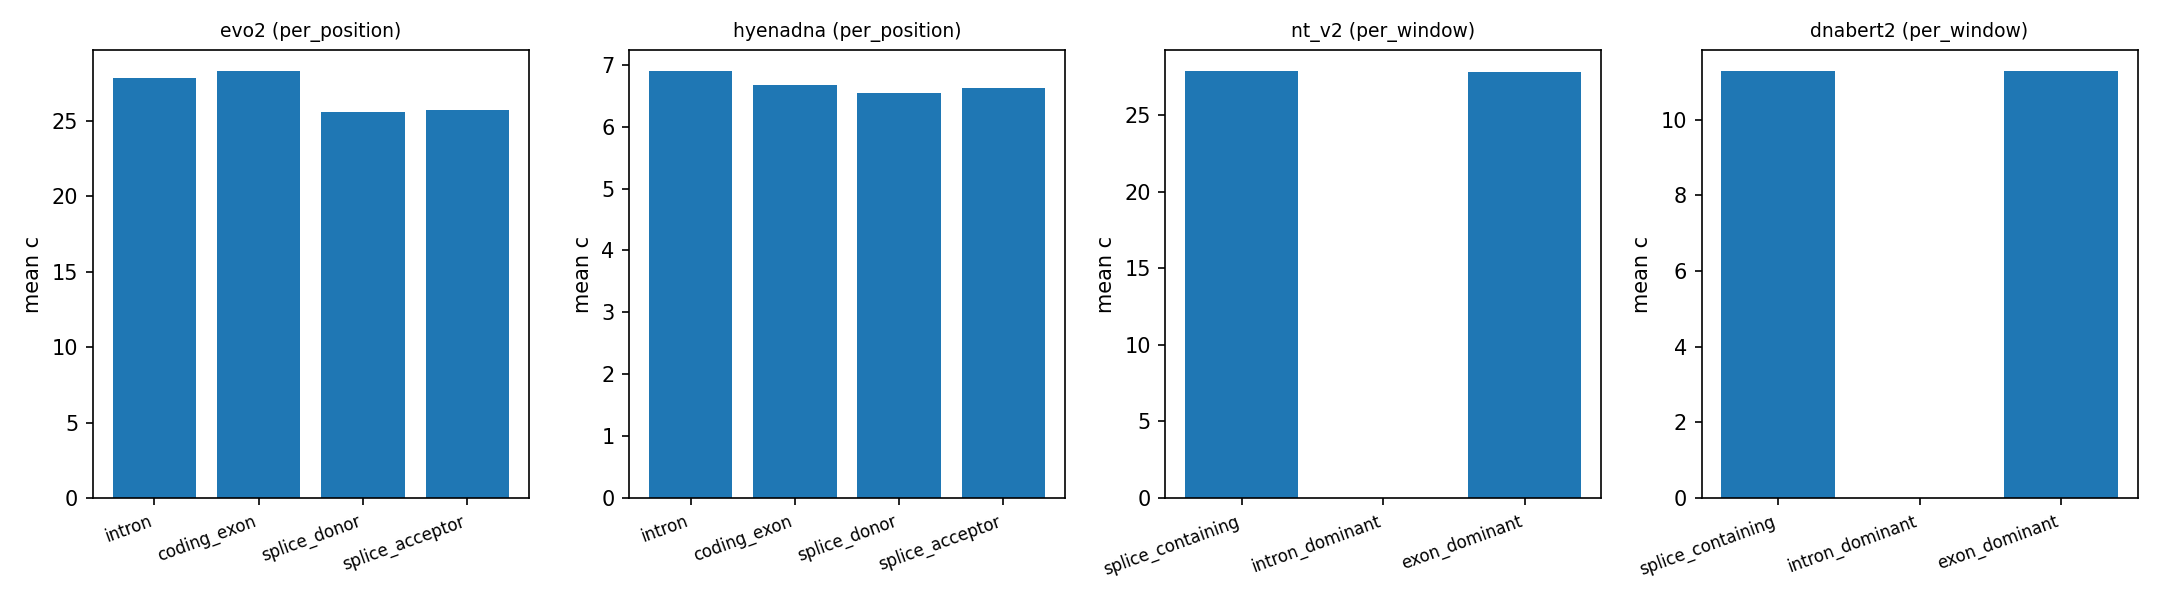
\includegraphics[width=0.95\linewidth]{figures/fig_appendix_b.png}
\caption{Per-context mean settling depth across the four genomic
foundation models. Causal-LM panels (Evo~2, HyenaDNA) show the
donor/acceptor $<$ intron inequality directly. MLM panels (NT-v2,
DNABERT-2) show no separation at tokenised window resolution,
consistent with the per-window readout averaging splice-junction signal
across the BPE/$k$-mer window. Underlying numbers:
\texttt{results/phase4/per\_model\_summary.json}.}
\label{fig:cross-arch-context}
\end{figure}

%%%%%%%%%%%%%%%%%%%%%%%%%%%%%%%%
% APPENDIX C — Reproducibility
%%%%%%%%%%%%%%%%%%%%%%%%%%%%%%%%
\section{Reproducibility}
\label{app:repro}

All experiments use random seed $42$ for cross-validation splits and
bootstrap resamples. The Evo~2 model lock is
\texttt{arcinstitute/evo2\_7b} at HF revision SHA
\texttt{bda0089f92582d5baabf0f22d9fc85f3588f6b58} (weights MD5
\texttt{359ef88ccac2a62644035578de8a7db4}). Data versions:
GRCh38 primary assembly (UCSC, MD5 locked); GENCODE v44 GTF
(per-chromosome filtered, persisted as \texttt{gffutils} SQLite);
PhyloP 100-way (UCSC); ENCODE SCREEN v3 cCRE catalog with ELS subset;
RepeatMasker hg38; GTEx v8 cis-eQTL pairs (\texttt{Whole\_Blood,
Brain\_Cortex, Liver, Lung} unioned); GWAS Catalog v1.0; ClinVar
2026-04-18. Software stack: \texttt{torch 2.4.1+cu124, evo2 0.3.0,
vortex 1.0.8, transformer-engine 2.14.0, transformers 4.49.0, scipy
1.13, scikit-learn 1.4}. Hardware: a single NVIDIA H200 (141\,GB).
Total compute: $\sim 20$ GPU-hours end-to-end. Code, dataset version
locks, and figure-generation scripts will be released at an anonymous
URL upon acceptance (an anonymized repository is provided as
supplementary material for review).

%%%%%%%%%%%%%%%%%%%%%%%%%%%%%%%%
% APPENDIX D — Per-layer ablation
%%%%%%%%%%%%%%%%%%%%%%%%%%%%%%%%
\section{Per-layer ablation table}
\label{app:per-layer}

Single-layer logistic-regression out-of-fold AUROC for each of the 32
layers under both lenses, on the same $8{,}008$-variant cohort and
10-fold stratified split (seed $=42$) used in
\S\ref{sec:variant-disruption}. Selected layers tabulated; full 32-row
table is released as \texttt{per\_layer\_auroc.csv}.

\begin{table}[h]
\caption{Selected per-layer AUROCs. Cosine and JSD lenses agree on the
U-shape but differ on which tap is sharpest: JSD concentrates
discriminative mass at the canonical tap $\ell=29$; cosine spreads it
across many taps, producing a much larger vector-vs-best-single-layer
gap.}
\label{tab:per-layer}
\centering
\small
\begin{tabular}{@{}llcc@{}}
\toprule
Layer & Block type & $\DDjsd$ AUROC & $\DDcos$ AUROC \\
\midrule
$0$  & embed                    & $0.605$ & $0.519$ \\
$7$  & \texttt{hcs} (shallow)   & $0.662$ & $0.595$ \\
$12$ & \texttt{hcm}             & $0.656$ & $0.555$ \\
$17$ & \texttt{attn}            & $0.723$ & $0.646$ \\
$24$ & \texttt{attn}            & $0.685$ & $0.612$ \\
$28$ & \texttt{hcs}             & $0.565$ & $0.698$ \\
$29$ (canonical tap) & \texttt{hcm}
                                & $\mathbf{0.794}$ (best JSD) & $0.604$ \\
$30$ (post-norm$-1$)  & ---     & $0.512$ & $\mathbf{0.729}$ (best cos) \\
$31$ (idle, see App.~\ref{app:architectural-quirk}) & ---
                                & $0.499$ (degen.) & $0.729$ ($=h_{30}$) \\
\midrule
32-d vector & all                 & $0.823$ & $0.844$ \\
\bottomrule
\end{tabular}
\end{table}

%%%%%%%%%%%%%%%%%%%%%%%%%%%%%%%%
% APPENDIX E — Q2 region detail and splice fine-profile
%%%%%%%%%%%%%%%%%%%%%%%%%%%%%%%%
\section{Largest Q2 region detail and splice fine-profile}
\label{app:q2-splice-profile}

The largest single contiguous Q2 region on chr22 spans coordinates
chr22:22{,}893{,}870--22{,}895{,}351 ($1{,}481$\,bp). Mean settling
depth within the region is $\bar c = 31.31$; mean PhyloP-100way is
$-0.63$. The region overlaps an annotated intron of an inactivated gene
model and is flanked by an ENCODE cCRE-ELS element $460$\,bp
downstream. No coding sequence intersects the region. We list this
single region as a representative case; $5{,}089$ additional Q2 regions
$\ge 100$\,bp are released as a BED file at \texttt{q2\_regions.bed} in
the supplementary materials.

On chr17 the donor profile reaches its mean settling-depth minimum at
position $+20$\,bp ($\bar c = 24.06$) and remains $\ge 1.5$ layers
below intronic baseline ($\bar c = 27.69$) out to $\pm 200$\,bp. On
the same chromosome the acceptor profile reaches its minimum at
$+50$\,bp ($\bar c = 23.33$) and similarly remains depressed beyond
$\pm 200$\,bp. On chr22 both donor and acceptor minima sit at coordinate
$0$ ($\bar c = 23.65$ and $23.64$ respectively). The asymmetry --- donor
minimum exonic-side, acceptor minimum intronic-side --- mirrors the
asymmetric splice-grammar features (branch point, polypyrimidine tract)
that lie predominantly on the intronic side of acceptors.

%%%%%%%%%%%%%%%%%%%%%%%%%%%%%%%%
% APPENDIX F — Detailed model specs
%%%%%%%%%%%%%%%%%%%%%%%%%%%%%%%%
\section{Detailed specifications of the four genomic foundation models}
\label{app:fm-specs}

\begin{table}[h]
\caption{Architectural specifications, tokenisation, per-window context,
runtime, and per-model $q_{70}$-calibrated $\gamma_{\cos}$ for the four
genomic foundation models compared in \S\ref{sec:cross-arch} and
Appendix~\ref{app:cross-arch}.}
\label{tab:fm-specs}
\centering
\footnotesize
\setlength{\tabcolsep}{4pt}
\begin{tabular}{@{}llcccll@{}}
\toprule
Model & Architecture & Layers & Hidden & Tokens / 6\,kb window
   & Wall-clock & $\gamma_{q_{70}}$ \\
\midrule
Evo~2~7B          & Hybrid Transformer + StripedHyena~2 & $32$ & $4096$
   & $6{,}000$ (1\,bp)         & reused      & $0.396$ \\
HyenaDNA-large-1m & Pure Hyena                          & $\phantom{0}8$ & $\phantom{0}256$
   & $6{,}001$ (1\,bp + BOS)   & $\sim 4$\,min    & $0.358$ \\
NT-v2~500M        & Transformer MLM ($k$-mer)           & $29$ & $1024$
   & $\phantom{0,}671$ ($k=6$, $\sim 4$\,kb) & $\sim 7.5$\,min  & $0.533$ \\
DNABERT-2~117M    & Transformer MLM (BPE)               & $12$ & $\phantom{0}768$
   & $\sim 600$ (BPE, $\sim 3$\,kb)        & $\sim 3$\,min    & $0.677$ \\
\bottomrule
\end{tabular}
\end{table}

%%%%%%%%%%%%%%%%%%%%%%%%%%%%%%%%
% APPENDIX G — Variant pathogenicity AUROC figure detail
%%%%%%%%%%%%%%%%%%%%%%%%%%%%%%%%
\section{Variant pathogenicity AUROC -- detailed panels}
\label{app:auroc-detail}

\begin{table}[h]
\caption{The 32-d trajectory dominates any single-layer feature. The
primary cosine lens reaches $0.844$ with 32 layers and only $0.729$ at
its best single tap -- a $+0.115$ gap. Bracketed numbers are
$1{,}000$-bootstrap $95\%$ confidence intervals.}
\label{tab:auroc}
\centering
\small
\begin{tabular}{@{}lccc@{}}
\toprule
Feature & dim. & Stratified 10-fold AUROC & LOGO-CV AUROC \\
\midrule
Best single-layer $\DDcos$ ($\ell=30$ tap) & $1$
   & $0.729$ $[0.717,\, 0.741]$
   & $0.726$ $[0.694,\, 0.758]$ \\
Best single-layer $\DDjsd$ ($\ell=29$ canonical tap) & $1$
   & $0.794$ $[0.781,\, 0.806]$
   & $0.787$ $[0.752,\, 0.821]$ \\
Evo~2 log-likelihood & $1$
   & $0.751$ $[0.738,\, 0.764]$
   & $0.793$ $[0.740,\, 0.846]$ \\
32-d $\DDjsd$ vector & $32$
   & $0.823$ $[0.813,\, 0.832]$
   & $0.821$ $[0.790,\, 0.853]$ \\
\textbf{32-d $\DDcos$ vector (primary)} & $32$
   & $\mathbf{0.844}$ $[0.831,\, 0.857]$
   & $\mathbf{0.843}$ $[0.811,\, 0.876]$ \\
Ensemble ($\Delta D + $ Evo~2 LL) & $33$
   & $0.861$ $[0.851,\, 0.871]$
   & $0.866$ $[0.832,\, 0.899]$ \\
\bottomrule
\end{tabular}
\end{table}

\begin{figure}[h]
\centering
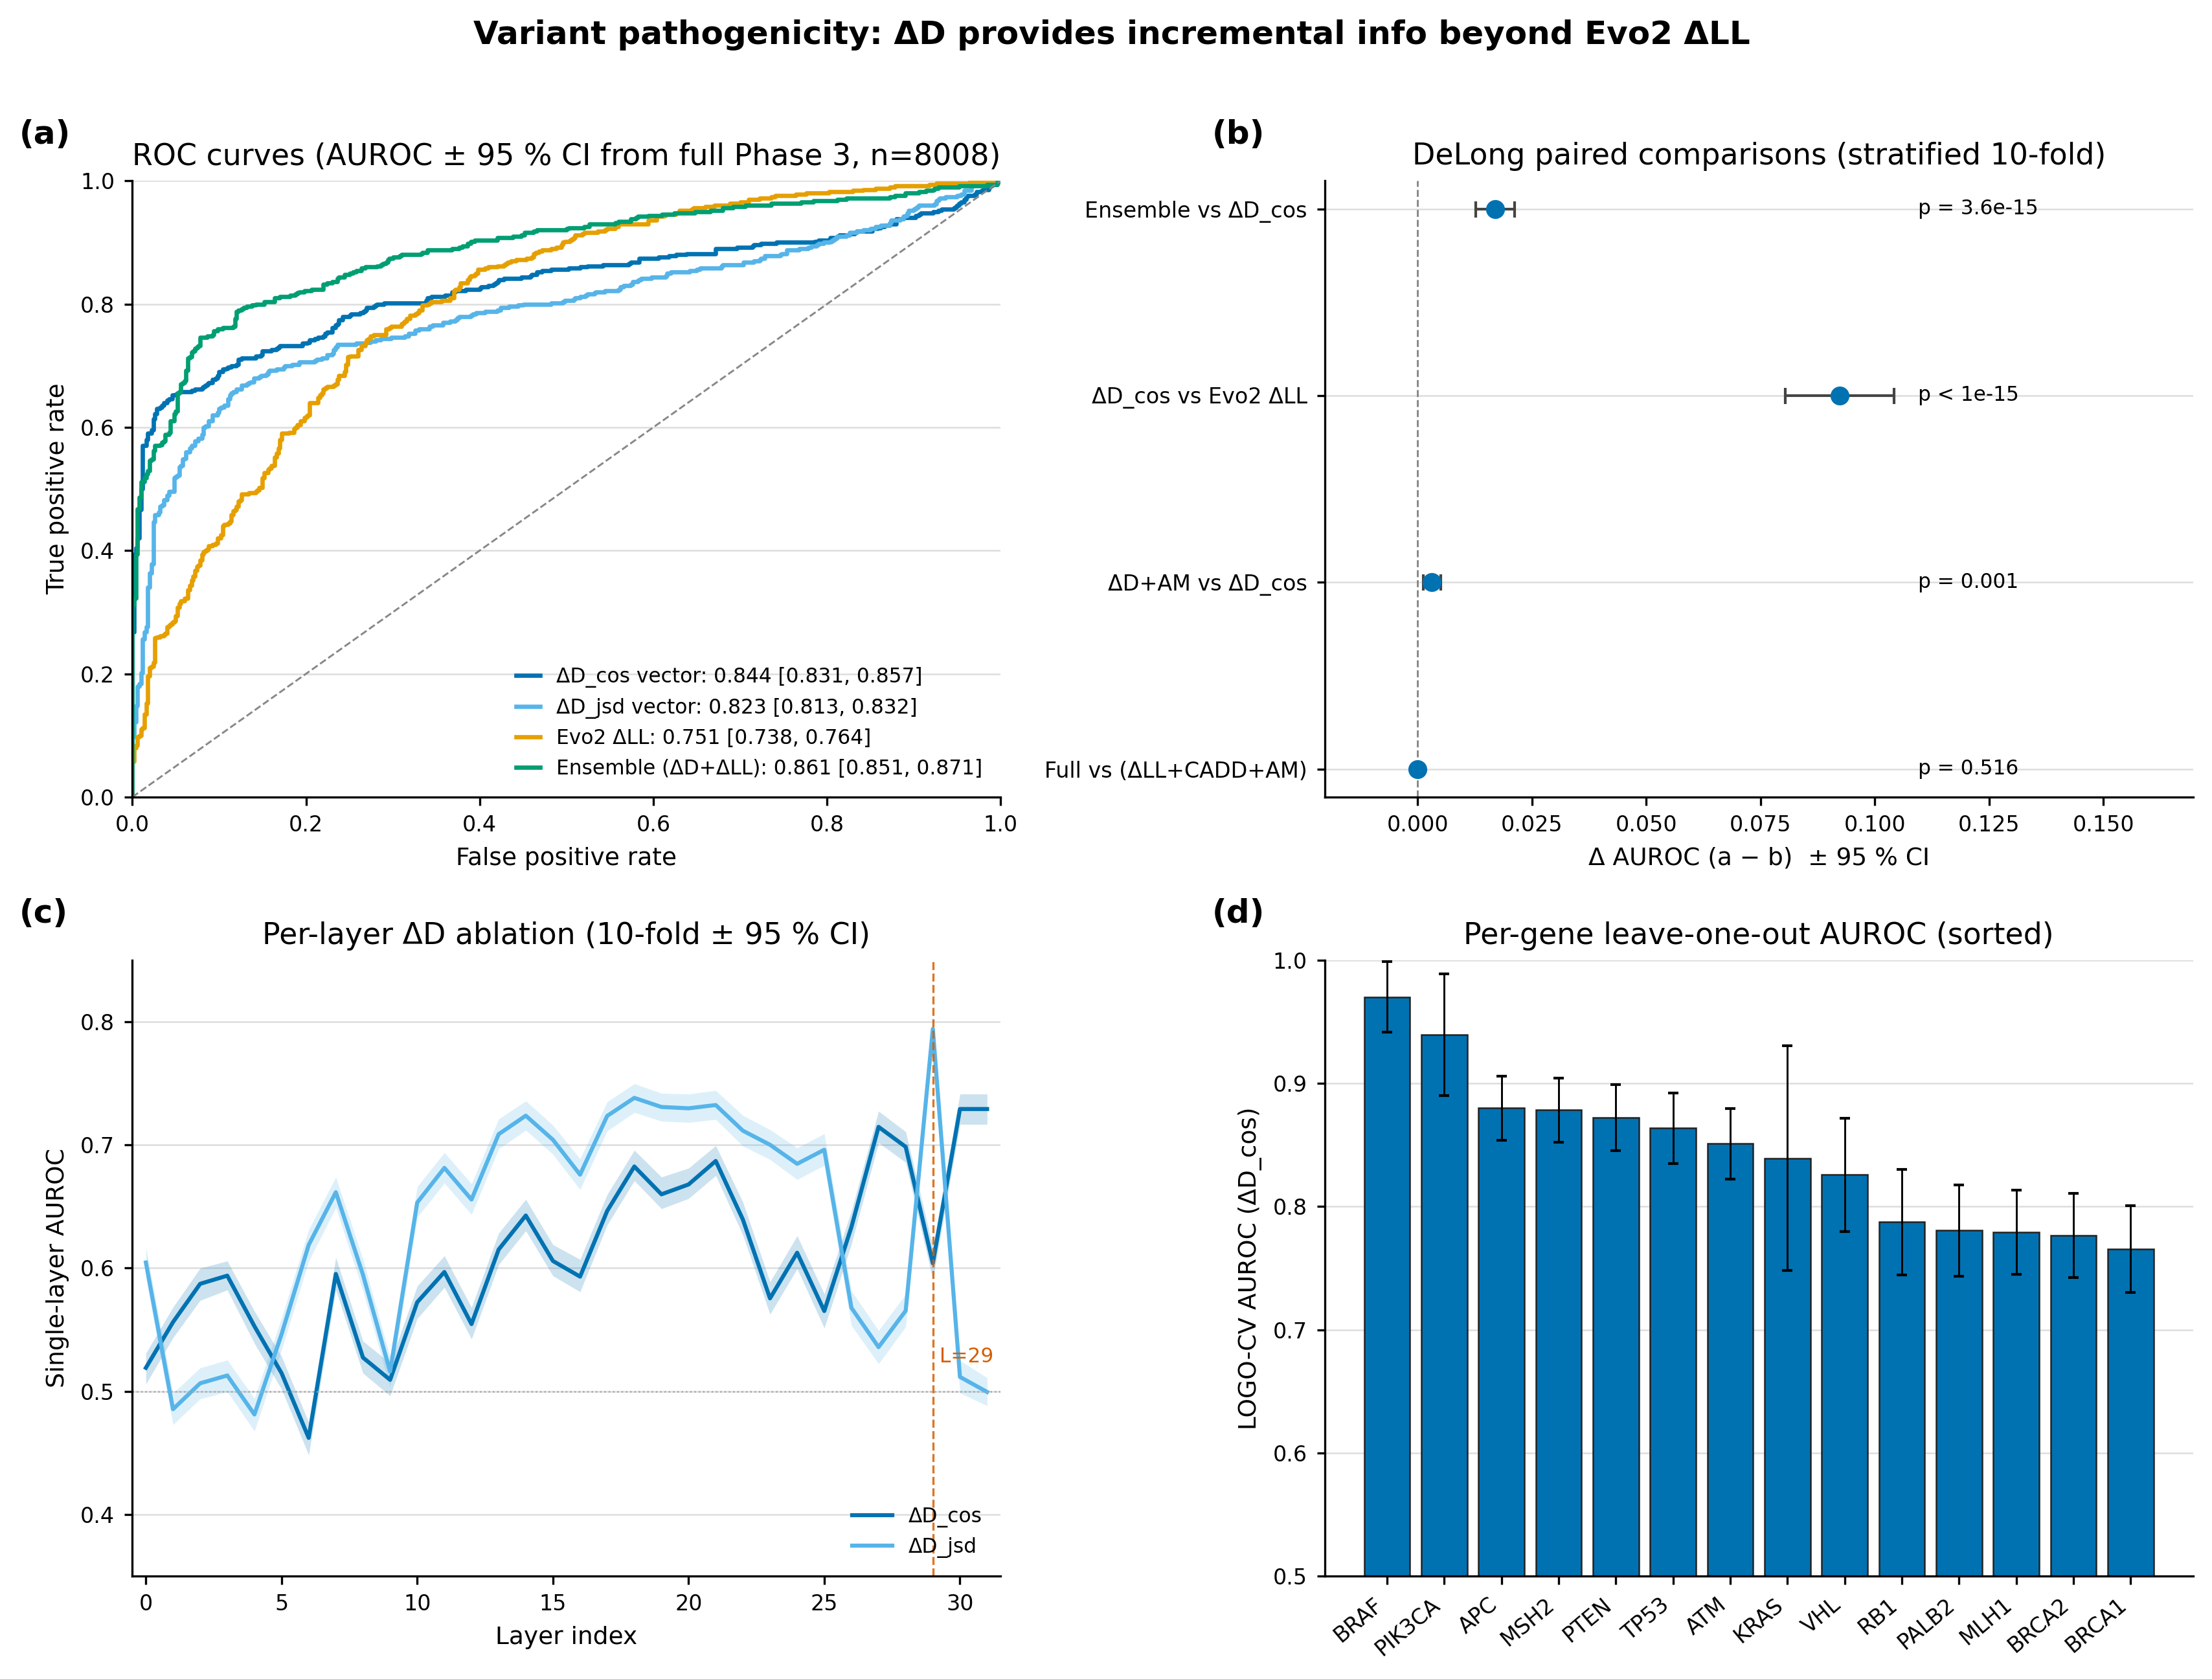
\includegraphics[width=0.95\linewidth]{figures/fig_auroc.png}
\caption{Variant pathogenicity discrimination on $8{,}008$ ClinVar
P/LP vs B/LB SNVs across 15 cancer-associated genes (the AUROC
numerical summary is Table~\ref{tab:auroc} above).
\textbf{(a)}~ROC curves for the four scoring features.
\textbf{(b)}~DeLong paired comparisons: $\Delta D$ adds significant
information beyond Evo~2 $\Delta\textrm{LL}$ ($p=3.6\times 10^{-15}$).
\textbf{(c)}~Per-layer single-feature AUROC across all 32 layers --
best single tap is $\ell=29$ for JSD; the 32-d vector beats it by
$+0.05$ to $+0.12$.
\textbf{(d)}~Leave-one-gene-out AUROC across 14 evaluable genes is
uniformly high ($\ge 0.77$).}
\label{fig:auroc}
\end{figure}

%%%%%%%%%%%%%%%%%%%%%%%%%%%%%%%%
% APPENDIX I — Splice canonical breakdown
%%%%%%%%%%%%%%%%%%%%%%%%%%%%%%%%
\section{Canonical vs.\ non-canonical splice motif breakdown}
\label{app:splice-canonical}

A finer dissection of the splice axis by motif class -- using the
genomic dinucleotides immediately downstream of the donor and upstream
of the acceptor -- reveals an unexpected ordering: \emph{non-canonical}
splice donors (AT-AC and other rare motifs, pooled $\bar c\!=\!25.13$,
$n\!=\!5{,}977$) converge \emph{earlier} than the dominant canonical
GT-AG donors ($\bar c\!=\!25.79$, $n\!=\!350{,}552$), while the minor
canonical GC-AG class is the deepest of the three
($\bar c\!=\!27.01$, $n\!=\!5{,}165$). The universality vs.\ intron
($\bar c\!=\!27.72$) holds for every splice class, but the within-class
ordering is the opposite of a naive ``stronger motif $\Rightarrow$
shallower recognition'' prior. The Cohen's $d$ between canonical GT-AG
and non-canonical donors is small ($\approx 0.05$), consistent with the
constrained branch-point and polypyrimidine context that flanks
non-canonical introns~\cite{wang2008splicecode,burge1998u12}; we
report the magnitudes honestly rather than over-interpret. The finding
replicates qualitatively on the 8-layer HyenaDNA-large at depth-normalised
scale.

%%%%%%%%%%%%%%%%%%%%%%%%%%%%%%%%
% APPENDIX H — Cross-architecture figure
%%%%%%%%%%%%%%%%%%%%%%%%%%%%%%%%
\section{Cross-architecture two-tier structure -- figure}
\label{app:crossarch-fig}

\begin{figure}[h]
\centering
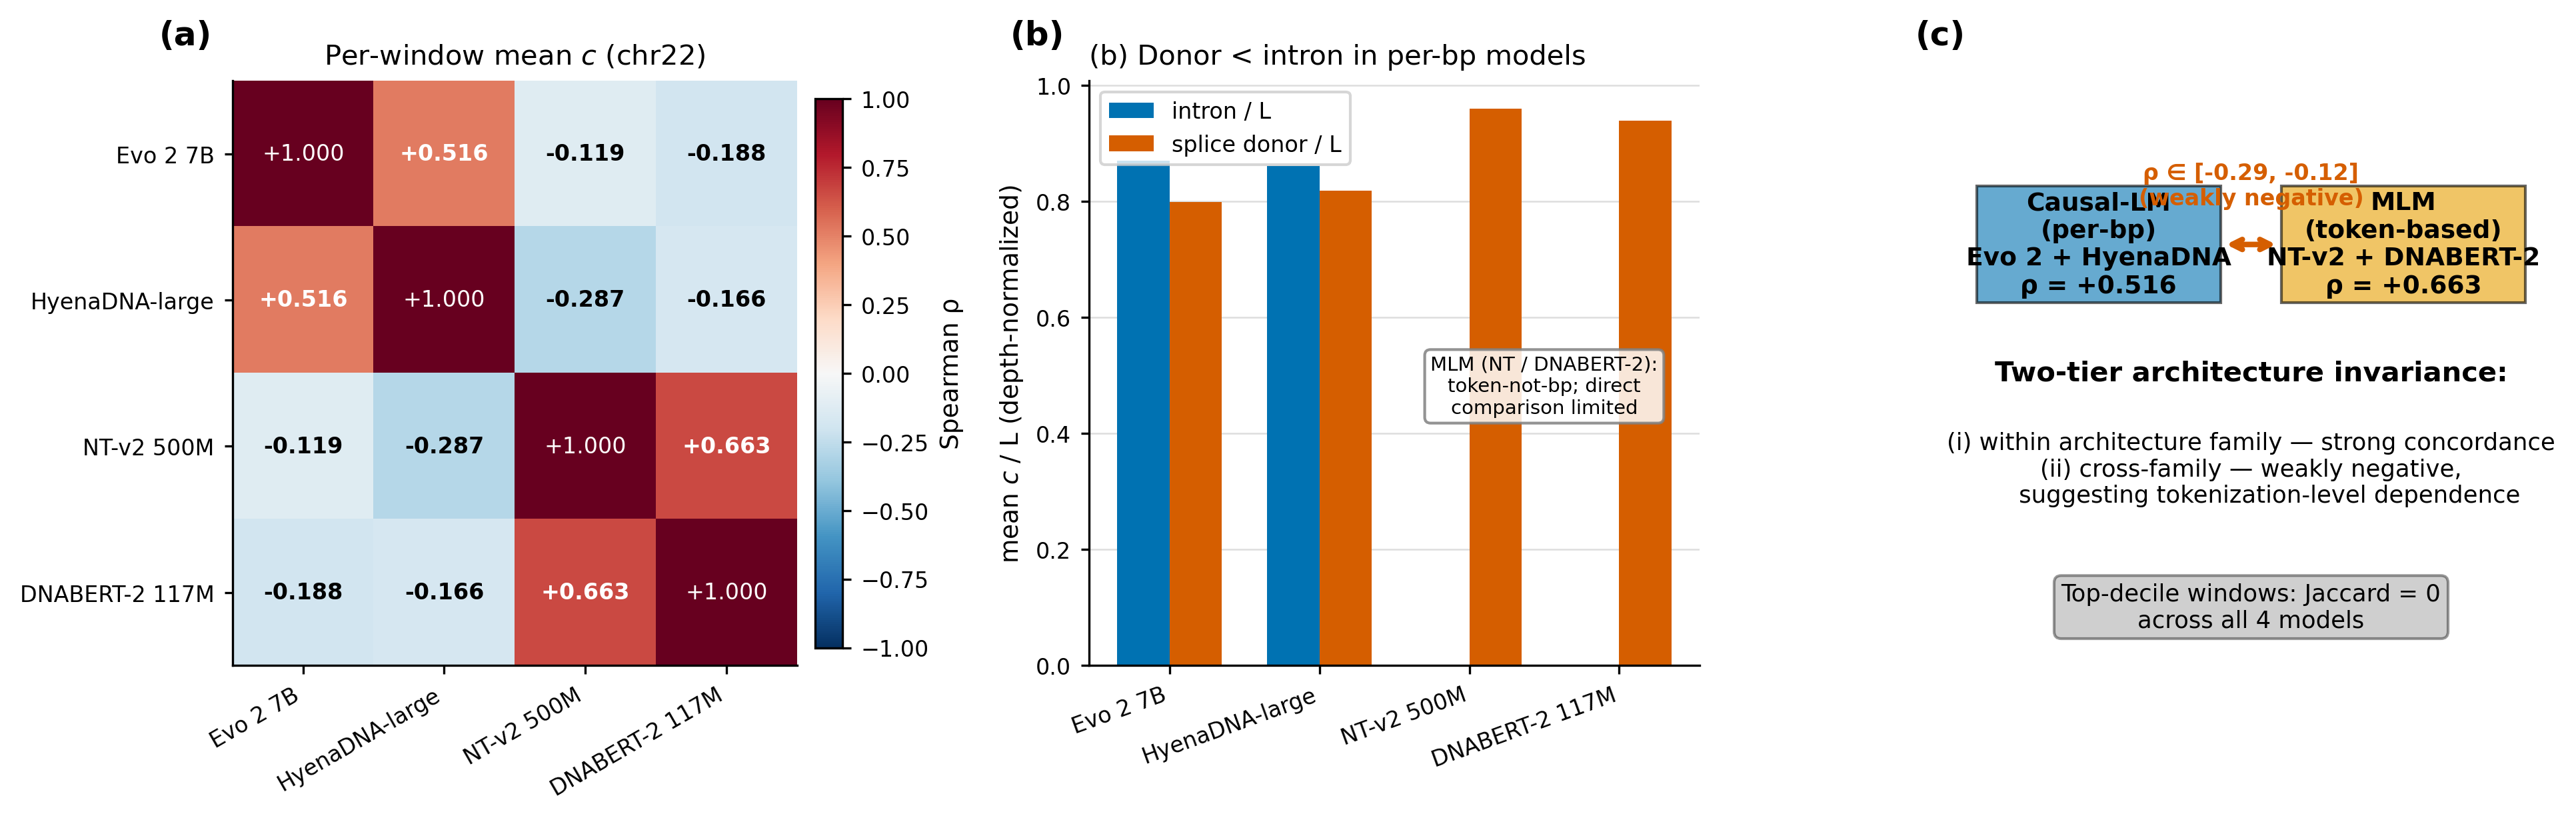
\includegraphics[width=0.95\linewidth]{figures/fig_crossarch.png}
\caption{Cross-architecture two-tier structure (numerical detail in
\S\ref{sec:cross-arch} body and Tables~\ref{tab:cross-arch-context},
\ref{tab:cross-arch-rho}). \textbf{(a)}~Pairwise Spearman $\rho$ of
per-window mean settling depth across four genomic foundation models
on chr22. \textbf{(b)}~Depth-normalised donor vs intron mean $c/L$:
per-bp causal-LMs (Evo~2, HyenaDNA) preserve donor $<$ intron;
tokenised MLMs (NT-v2, DNABERT-2) tokenise at window level and
therefore show no per-position separation. \textbf{(c)}~Schematic of
the two-tier structure with the within/cross-family $\rho$ values.}
\label{fig:cross-arch}
\end{figure}

\end{document}
